\section{Speicherhierarchie}

\begin{center}
    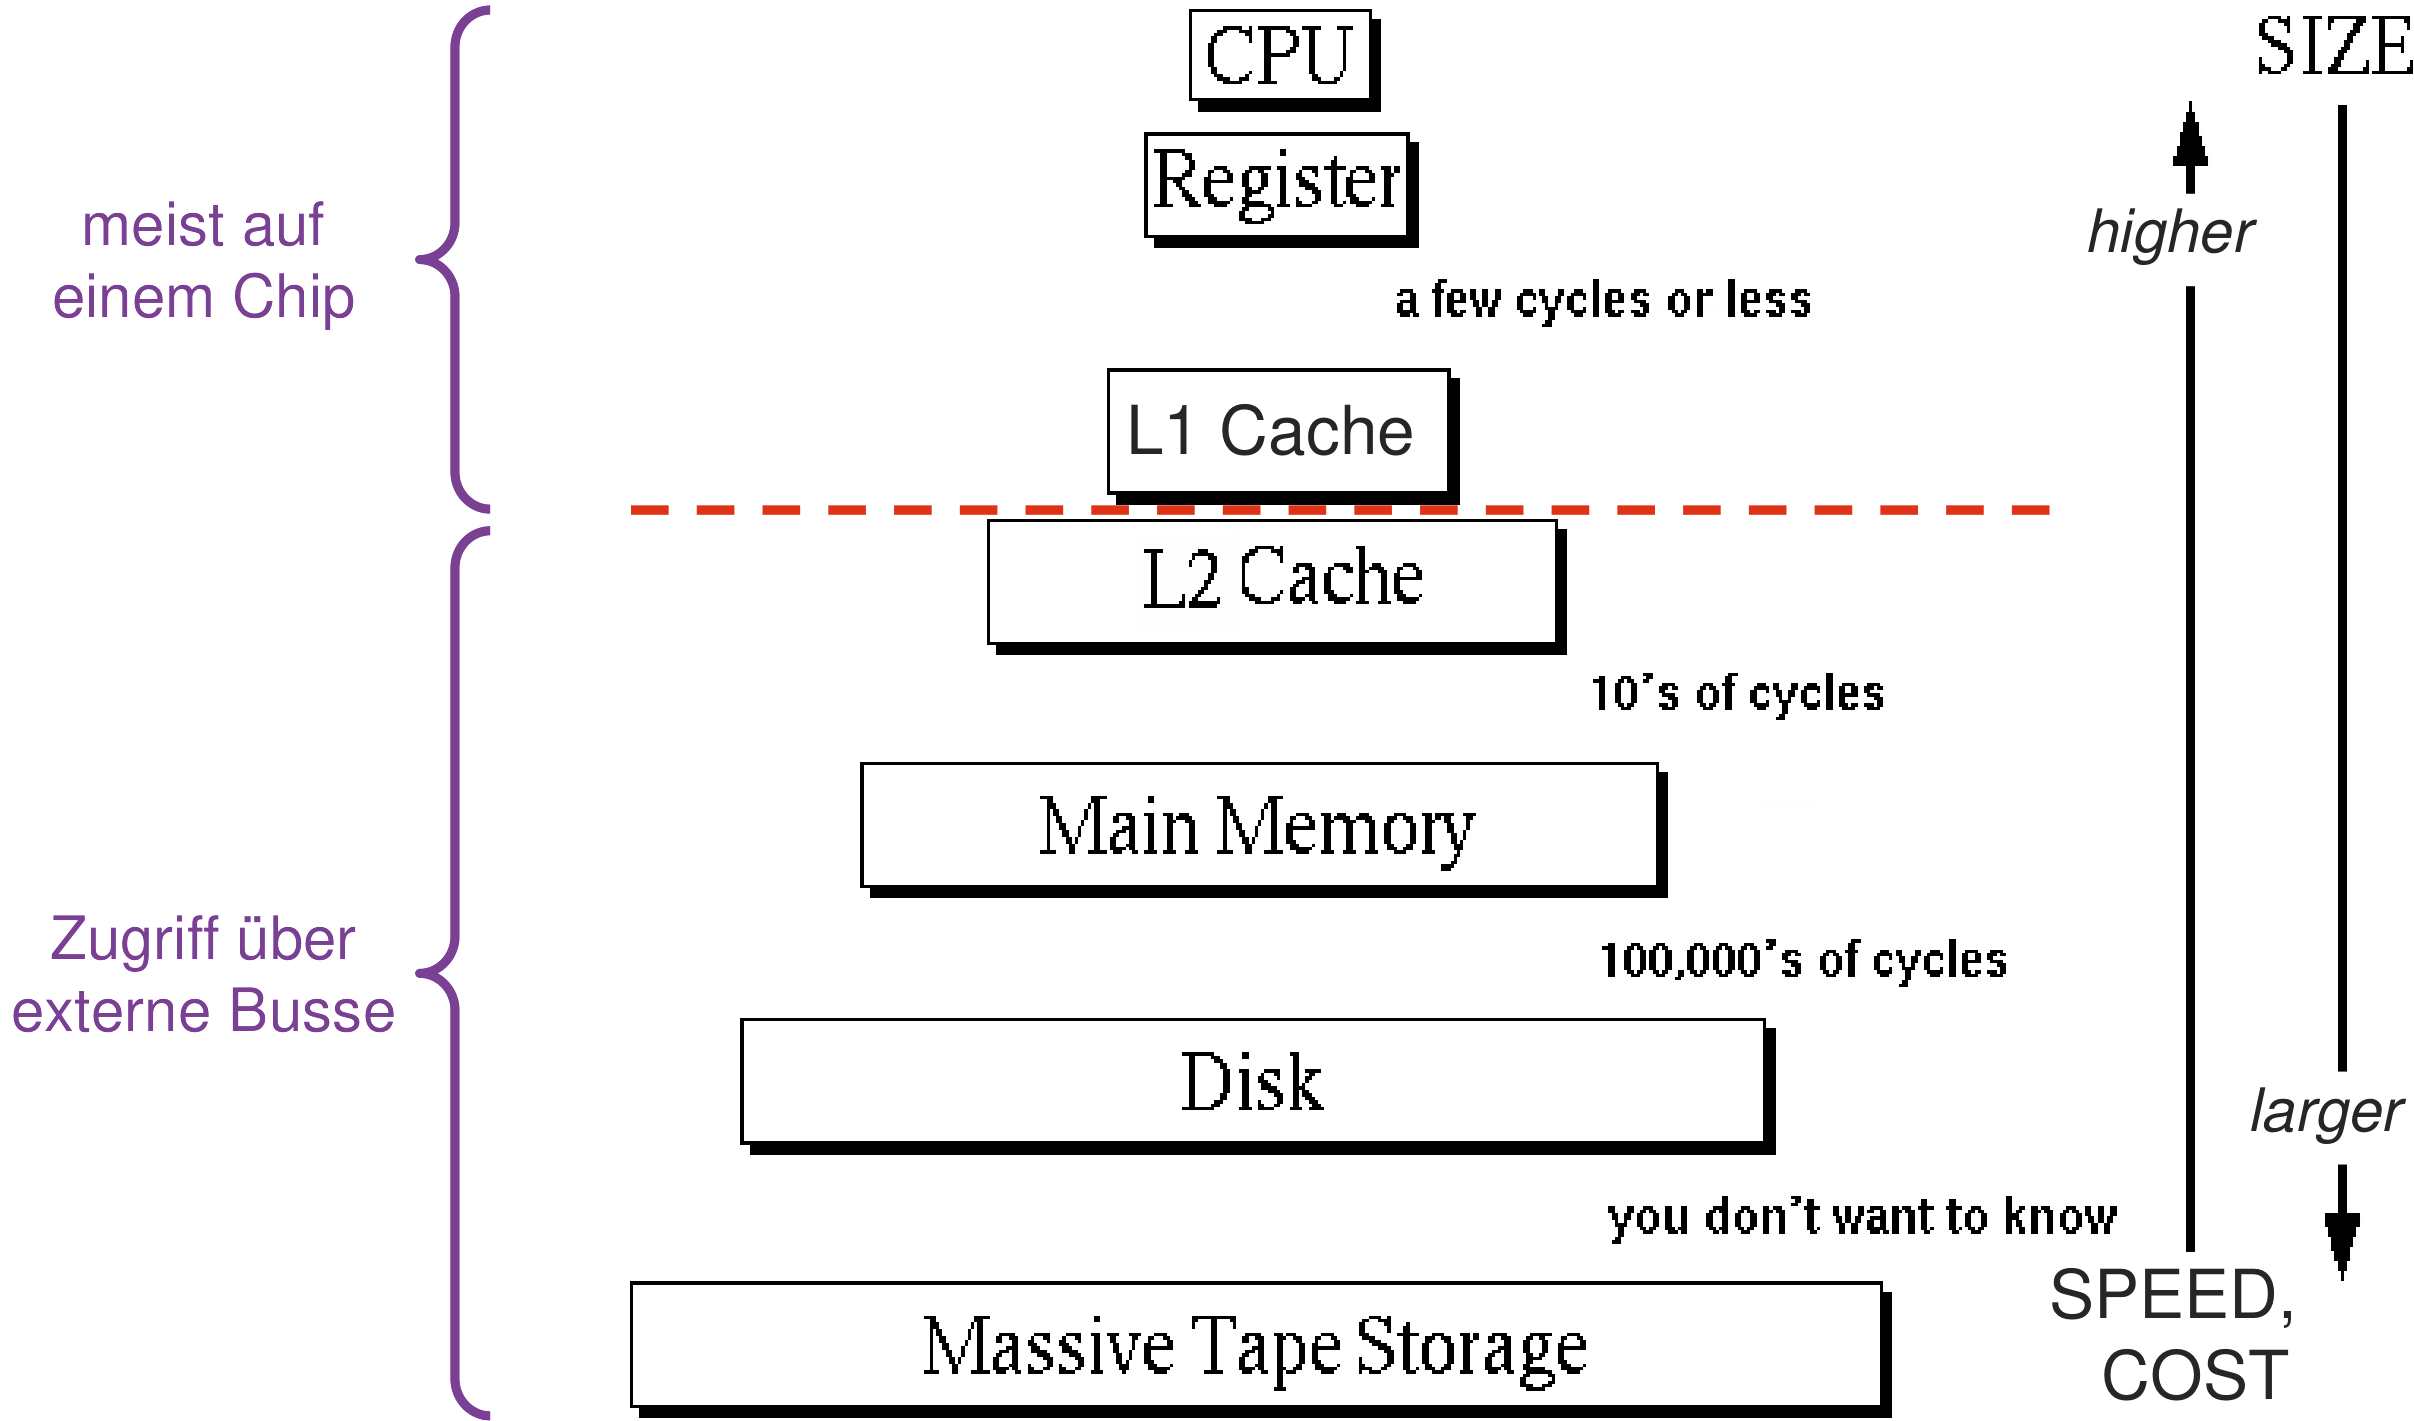
\includegraphics[width=.8\linewidth]{Speicherhierarchie.png}
\end{center}

\subsection{Cache-Speicher}

\begin{itemize}
    \itemsep-.5em 
    \item L1-Cache: auf gleichem Chip wie CPU, arbeiten mit der CPU-Geschwindigkeit, typisch bis etwa 128 KByte
    \item L2-, L3-Cache: ausserhalb des CPU-Chips, wesentlich langsamer als L1-Cache, L2 typisch 256 KByte bis mehrere MByte
\end{itemize}

Es gilt das Lokalitätsprinzip: Kopien von häufig (zeitliche Lokalität der Programmausführung) oder miteinander (örtliche Lokalität) benötigten Instruktionen/Daten aus dem Hauptspeicher.
Cache-Speicher (Daten, Adressen) und Cache-Controller (Steuersignal); Cache für den Prozessor versteckt, Programm läuft mit und ohne Cache.

Das Cache Directory ist als Assoziativ-Speicher aufgebaut, Content Addressable Memory (CAM):

\begin{center}
    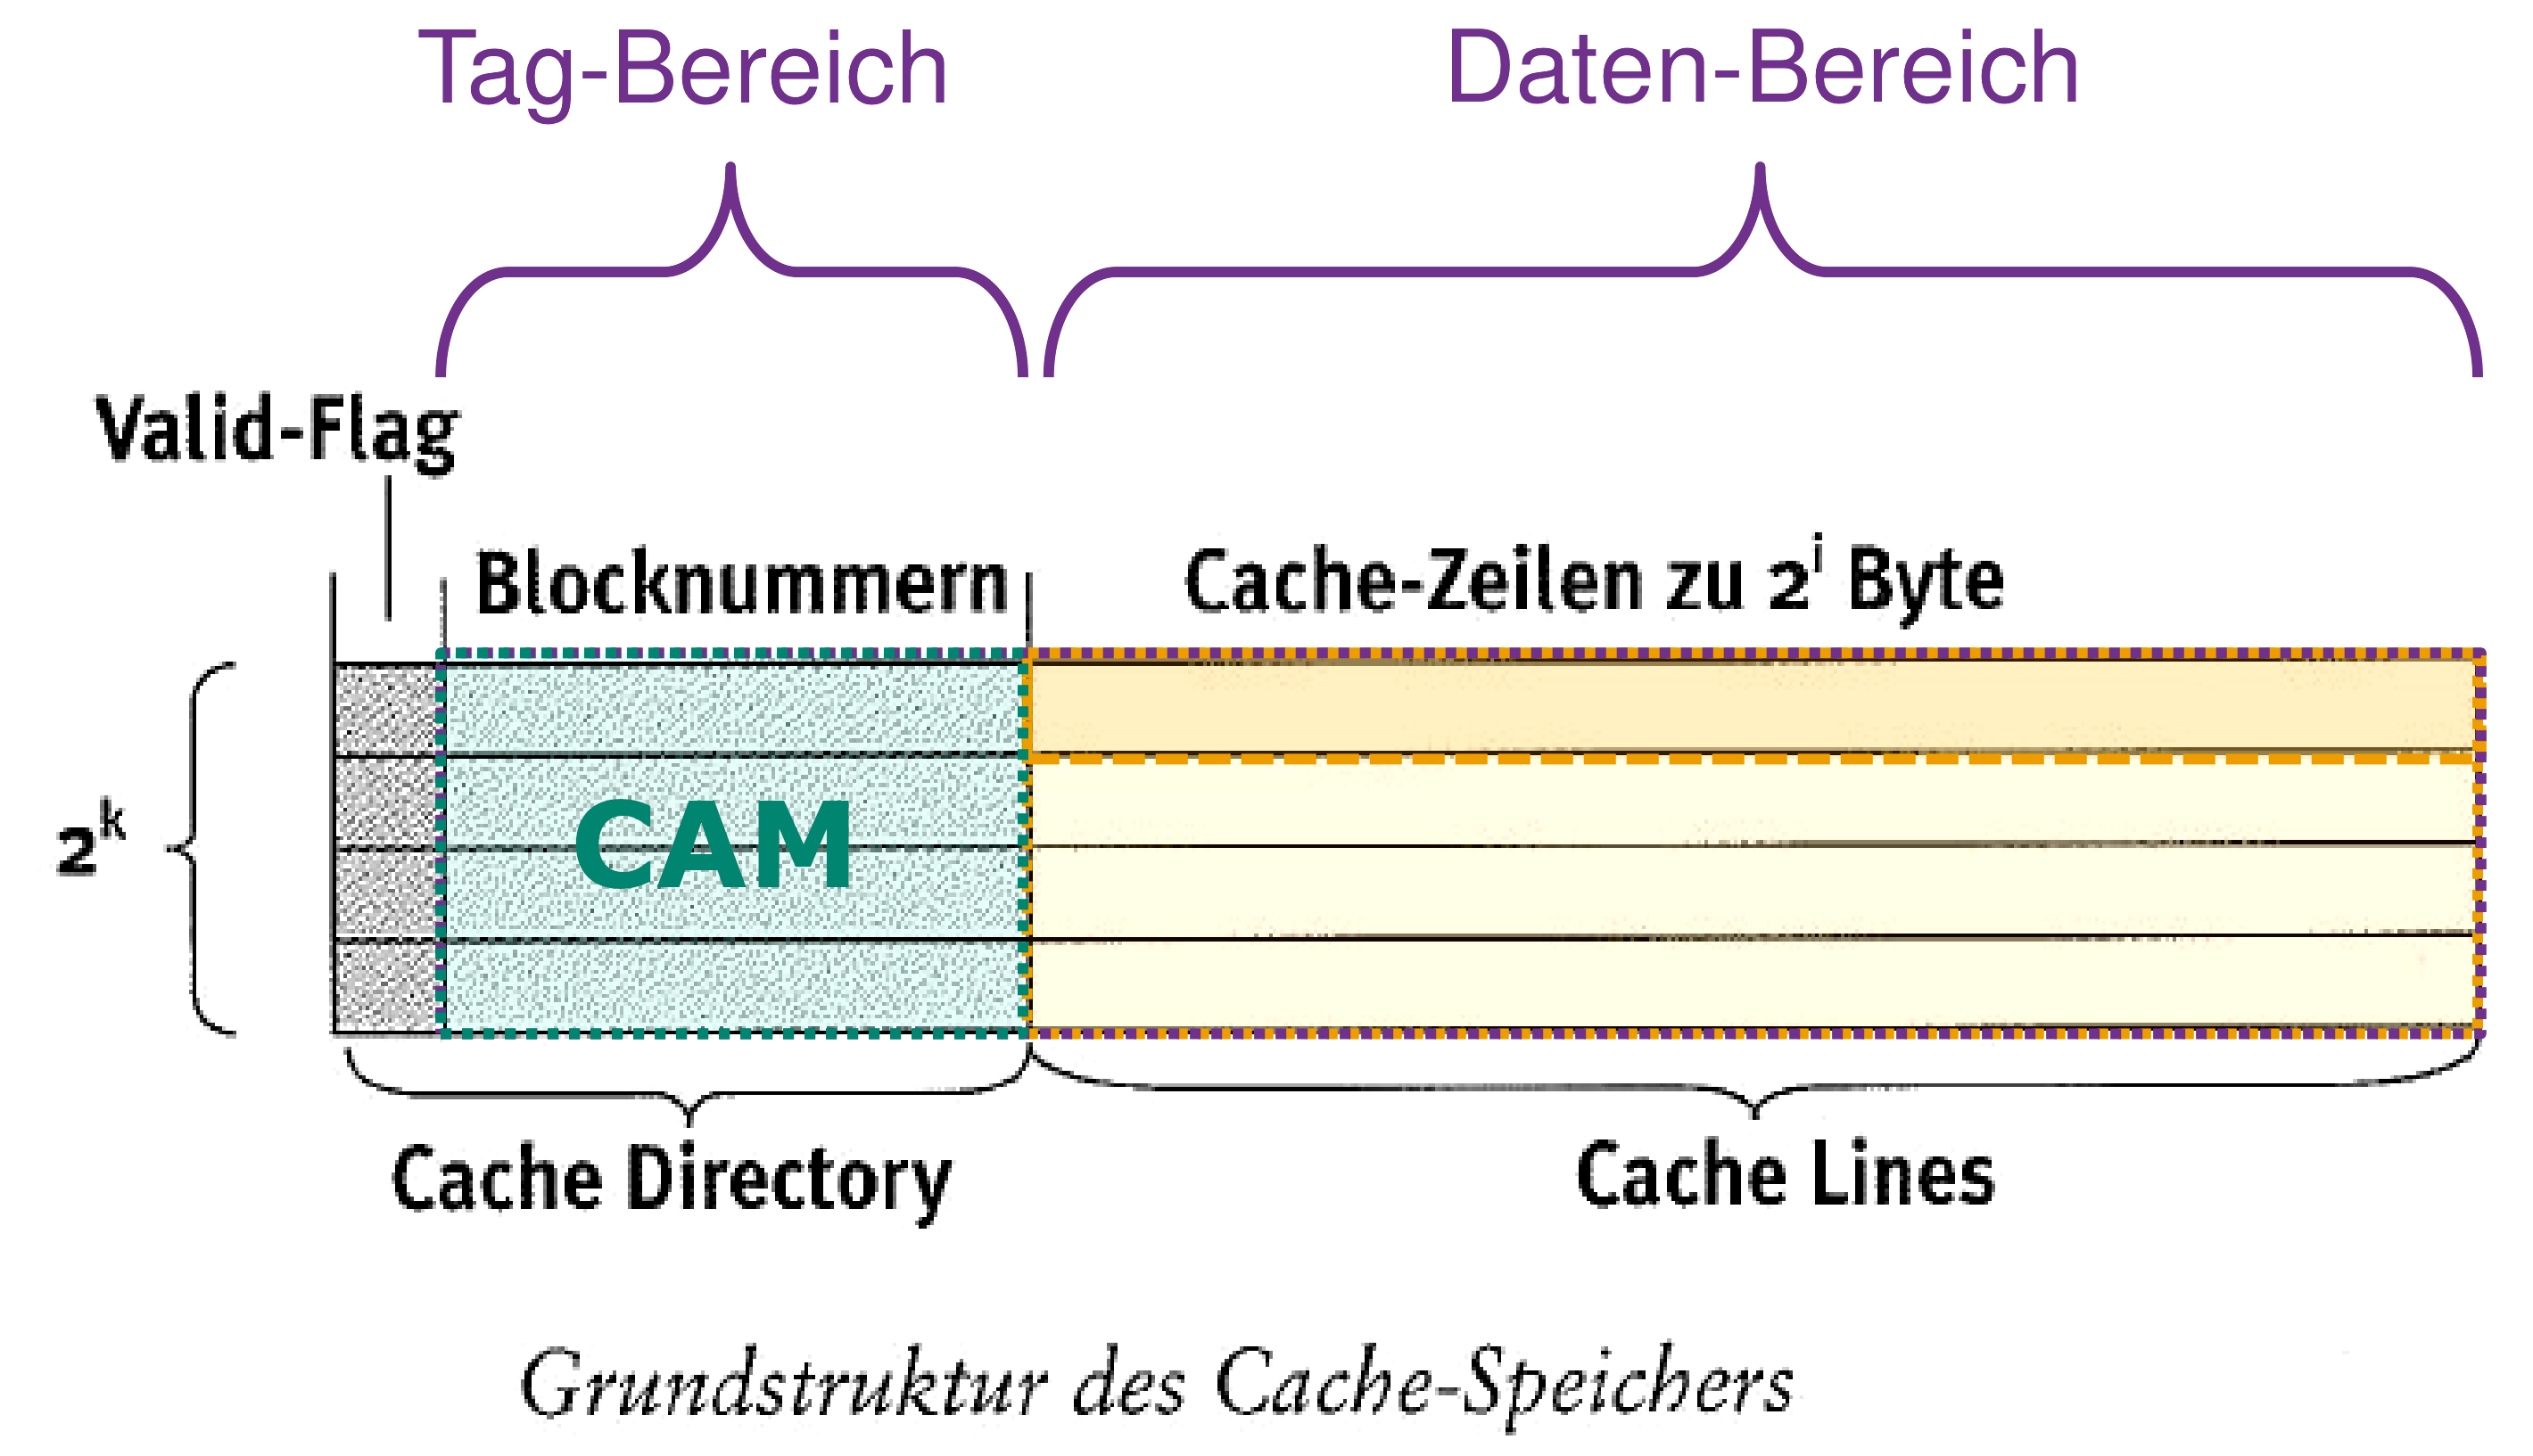
\includegraphics[width=.8\linewidth]{cache_cam.png}
\end{center}

\subsection{Cache Organisation}

\subsubsection{Voll-assoziativ}

Die Dateneinheit kann sich an beliebiger Stelle im Cache befinden.
Beim CAM-Zugriff sind $2^k$ Vergleiche gleichzeitig in der Cache-Hardware durchzuführen.

Übung: Kontinuierlich von Vorne her aufgefüllt (Start Zeile 0)

Cache Grösse: \formula{$2^{k+i}$}
Anzahl Zeilen: \formula{$2^k$}
Zeilen-Grösse: \formula{$2^i$}

\begin{center}
    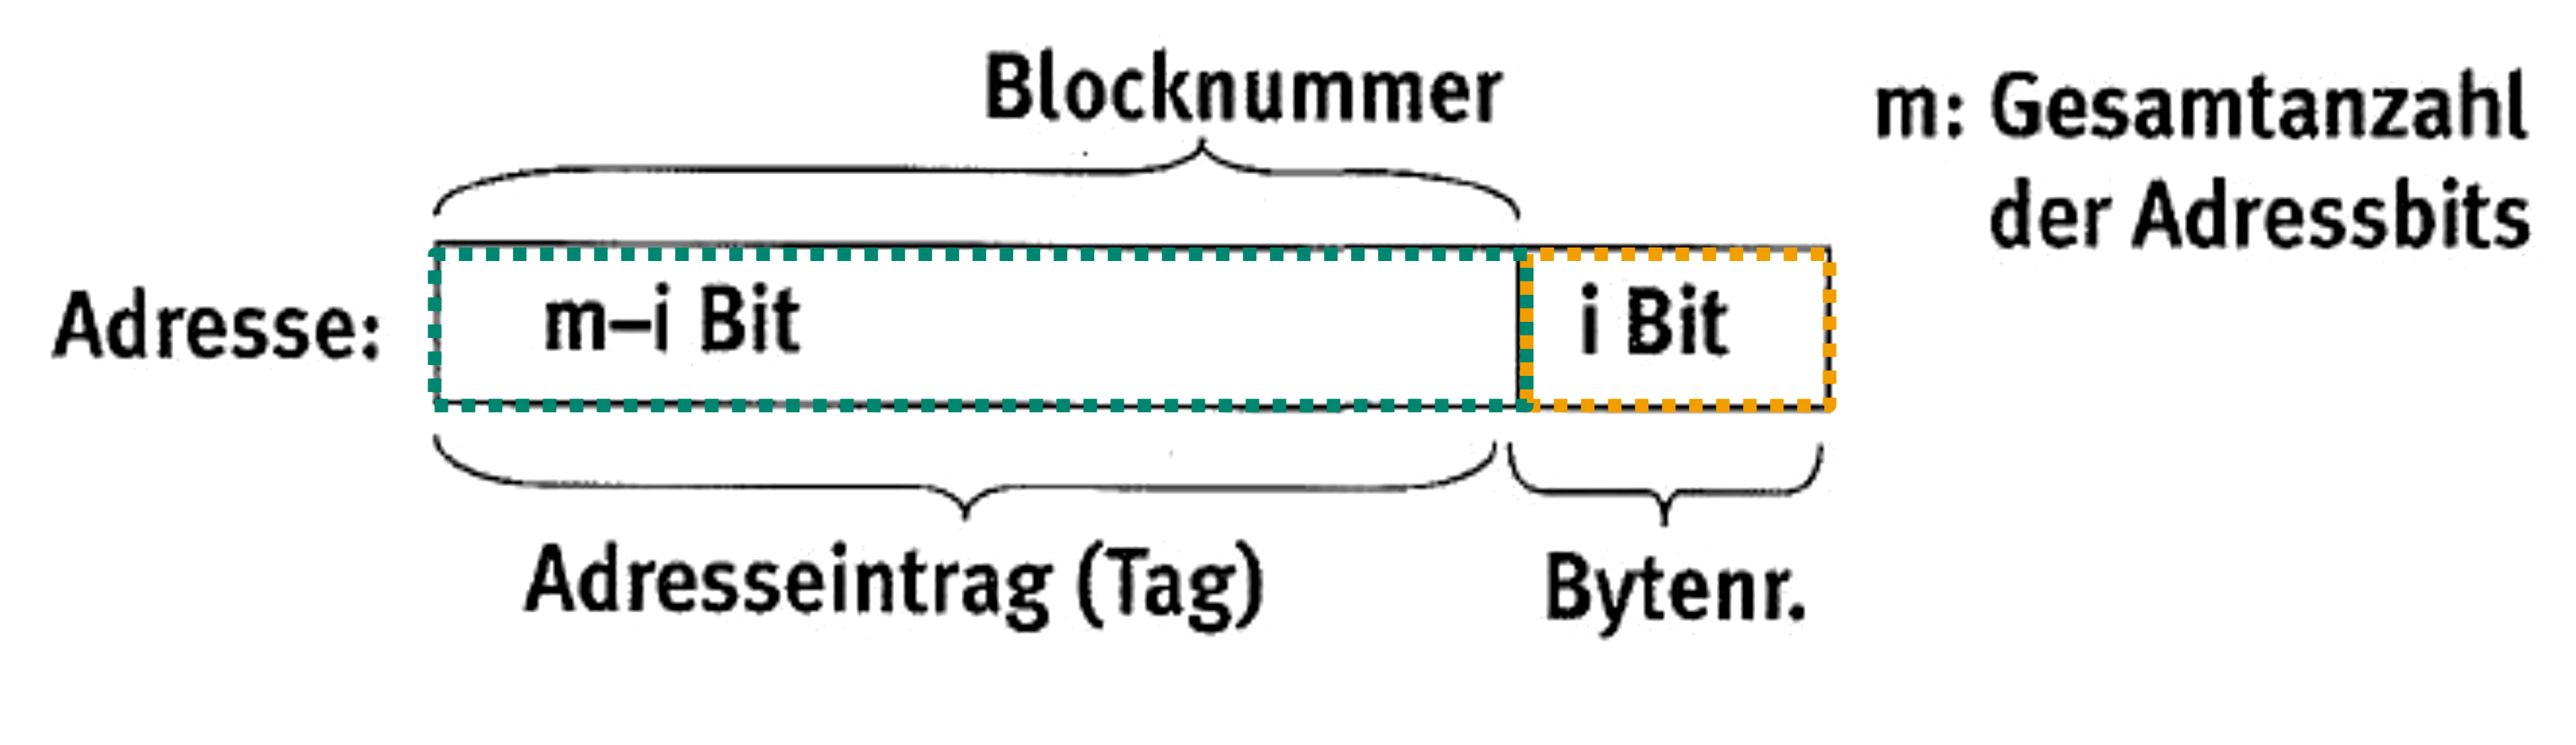
\includegraphics[width=.8\linewidth]{cache_vollassoziativ.png}
\end{center}

\subsubsection{Einweg-assoziativ}

Auch \textit{Direct-Mapped Cache} gennant. Eindeutige Abbildung zwischen den Blocknummern und den Cache-Zeilennummern.
Nur noch ein Adressvergleich nötig. Ungünstige Folge von Speicherzugriffen kann ein sehr häufiges Nachladen ergeben.

Übung: Tags in gleicher Zeile jeweils Überschreiben.

Cache Grösse: \formula{$2^{k+i}$}
Anzahl Zeilen: \formula{$2^k$}
Zeilen-Grösse: \formula{$2^i$}

\begin{center}
    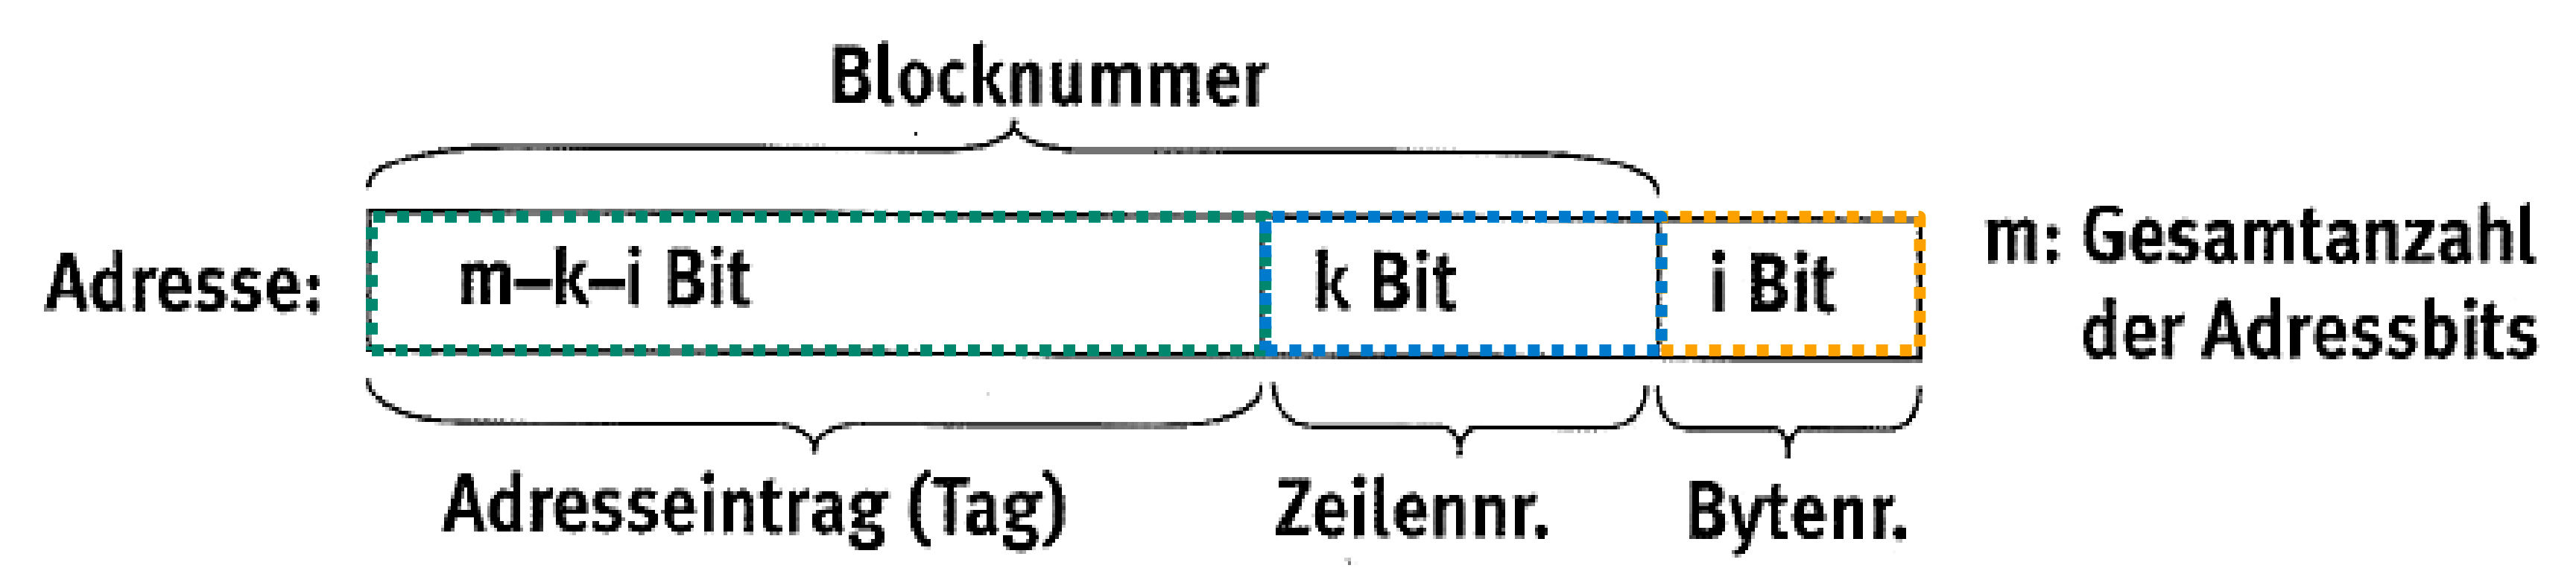
\includegraphics[width=.8\linewidth]{cache_einwegassoziativ.png}
\end{center}

\subsubsection{N-weg assoziativ}

Pro Zeilennummer stehen mehrere Cache-Zeilen zur Auswahl. Jede Cache-Zeile wird n-mal dupliziert.
Es sind insgesamt n Adressvergleiche nötig.

Übung: Wenn Zeile bereits mit anderem Tag belegt, in nächsten Block (n-Way) schreiben.

Cache Grösse: \formula{$n \cdot 2^{k+i}$}
Anzahl Zeilen: \formula{$2^k$}\\
$n$ Blöcke à Zeilen-Grösse: \formula{$2^i$}

\subsection{Ersetzungsstrategien}

\begin{itemize}
    \itemsep-.5em 
    \item LRU (Least Recently Used)
    \item Random Strategie
    \item FIFO (First In First Out)
    \item LFU (Least Frequently Used)
    \item Pseudo-LRU (Siehe Bild)
\end{itemize}

\begin{center}
    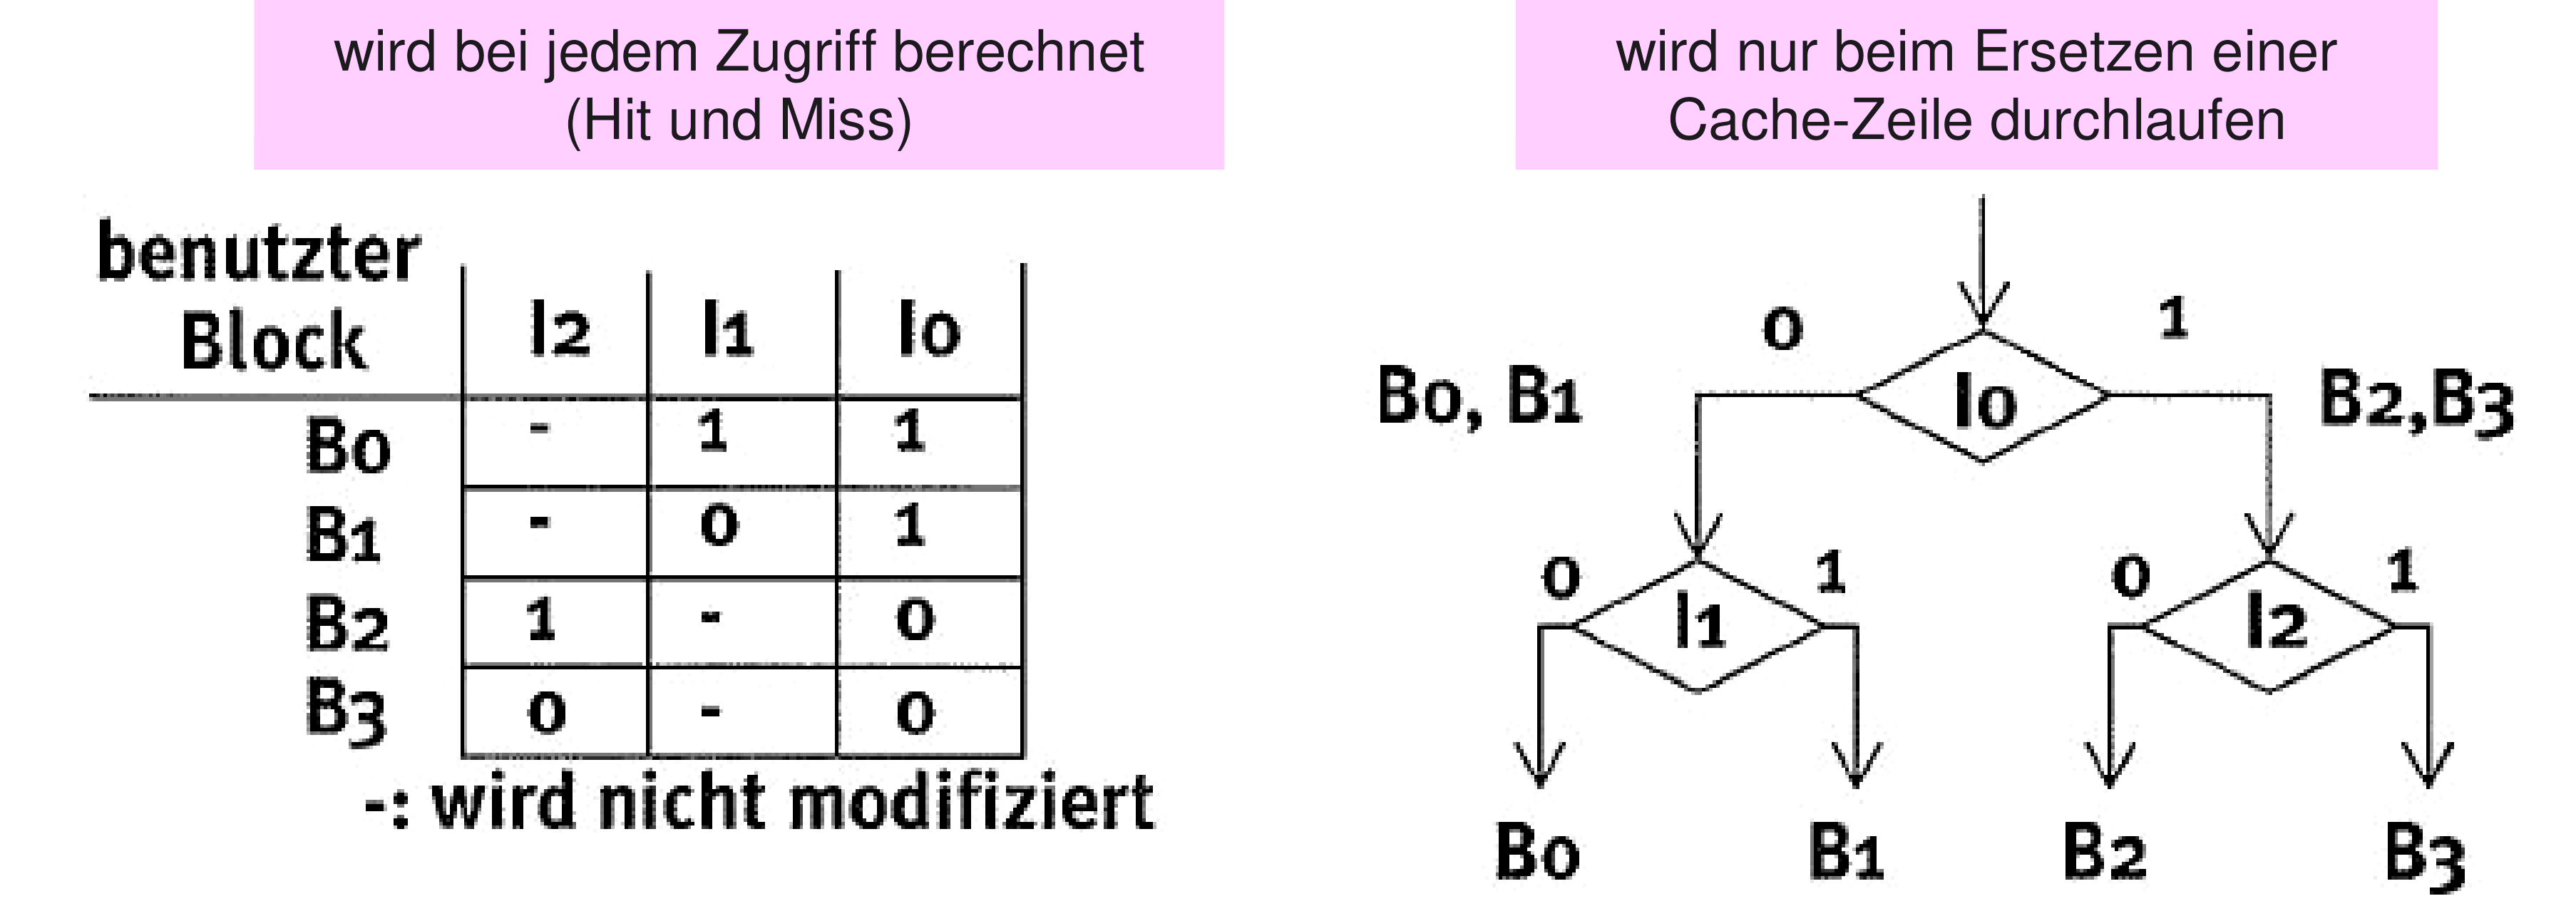
\includegraphics[width=\linewidth]{PLRUexample.png}
\end{center}

\subsection{Schreiben}

\begin{center}
    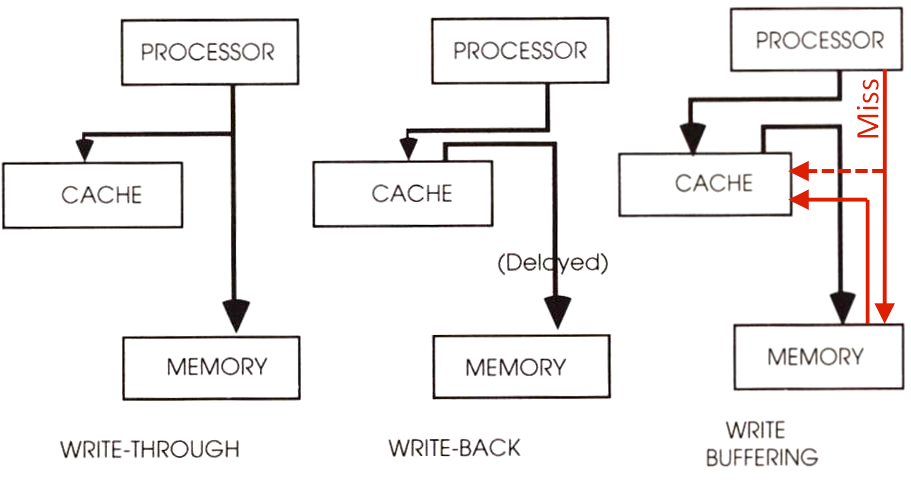
\includegraphics[width=\linewidth]{Cache_Schreiben.png}
\end{center}

\subsubsection{Write Through (Store Through)}

Bei jedem Schreibzyklus werden die Daten in den Hauptspeicher zurückgeschrieben.

\subsubsection{Write Back (Copyback, Store In)}

Bei einem Write-Hit wird nur der Cache-Inhalt neu geschrieben.
Zurückschreiben aller geänderten Cache-Zeilen in den Hauptspeicher wird
durch eine Maschineninstruktion oder Hardware-Signal veranlasst bzw. beim Ersetzen der jeweiligen Cache-Zeile.

\subsubsection{Write Allocate}

Möglichkeiten bei Write-Miss:
\begin{itemize}
    \itemsep-.5em 
    \item No-Write Allocate: Write-Miss verändert Cache nicht; stattdessen direktes Schreiben in Hauptspeicher
    \item Write Allocate: Nachladen der Cache-Zeile (= Read-Miss); danach Verfahren wie bei Write-Hit
\end{itemize}

Typische Kombinationen:
\begin{itemize}
    \itemsep-.5em 
    \item Write Back Cache mit Write Allocate
    \item Write Through Cache mit No-Write Allocate
\end{itemize}

\subsection{Performance}

\formula{$\mathit{Memory\, stall\, cycles} = \mathit{Number\, of\, misses} \cdot \mathit{Miss\, penalty}$}
\formula{$= \mathit{IC} \cdot \dfrac{\mathit{Misses}}{Instructions} \cdot \mathit{Miss\, penalty} $}
\formula{$= \mathit{IC} \cdot \dfrac{\mathit{Memory\, accesses}}{Instructions} \cdot \mathit{Miss\, rate} \cdot \mathit{Miss\, penalty} $}

\formula{$T_{eff} = T_{Hit} + r_{Miss} \cdot A_{Miss}$}

\unitText{$T_{eff}$}{Durchschnittliche Zugriffszeit}{s, Clocks}\\
\unitText{$T_{Hit}$}{Cache zugriffszeit}{s, Clocks}\\
\unitText{$r_{Miss}$}{Miss-Rate im Cache}{\%}\\
\unitText{$A_{Miss}$}{Zusätzlicher Zeitaufwand bei Nichttreffer}{s, Clocks}

\subsection{Cache-Friendly Code}

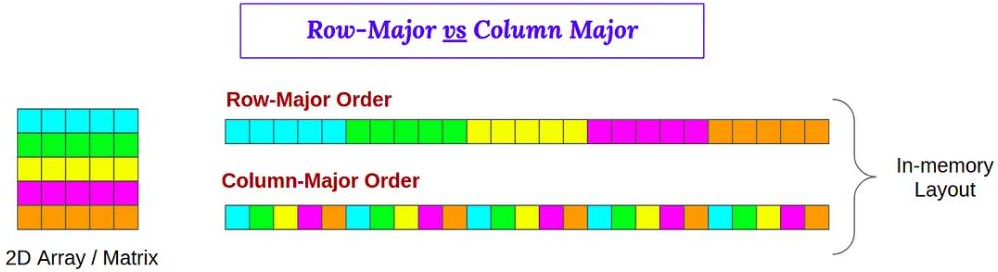
\includegraphics[width=\linewidth]{cache_friendly_code_2.png}
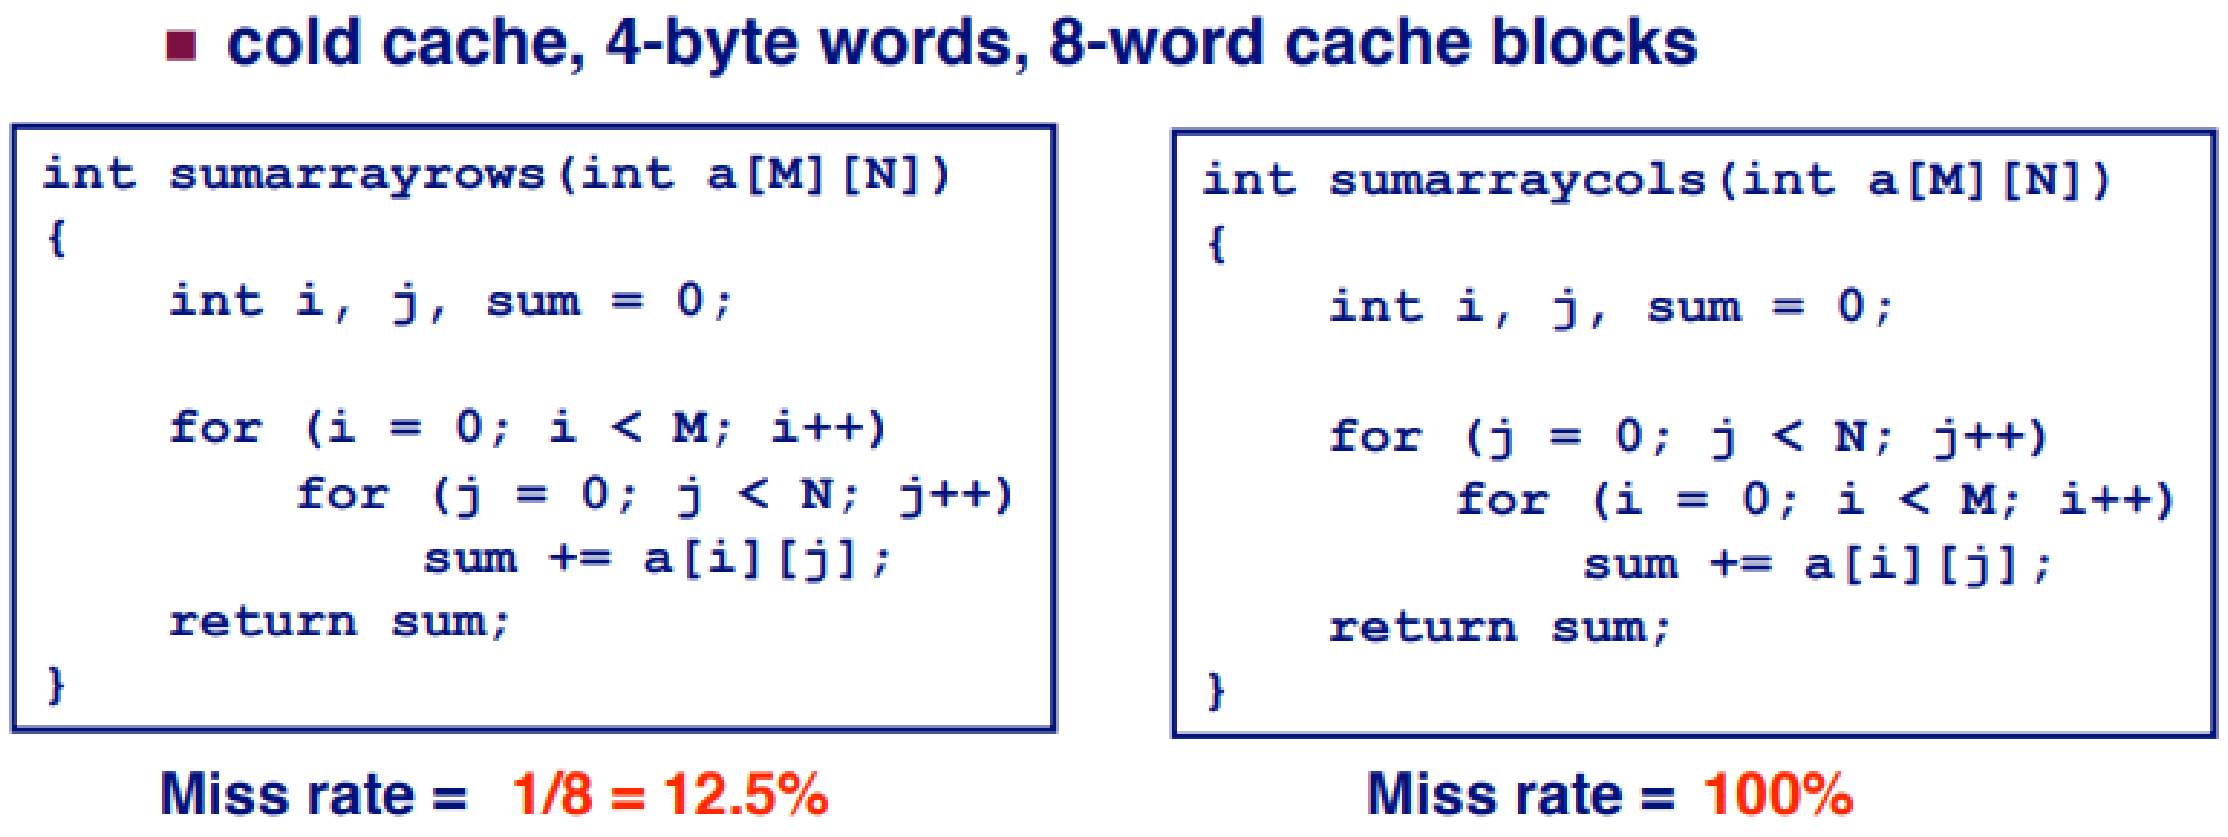
\includegraphics[width=\linewidth]{cache_friendly_code_1.png}